\section{Retrofit gains on paired visits}

\begin{figure*}[t]
  \centering
  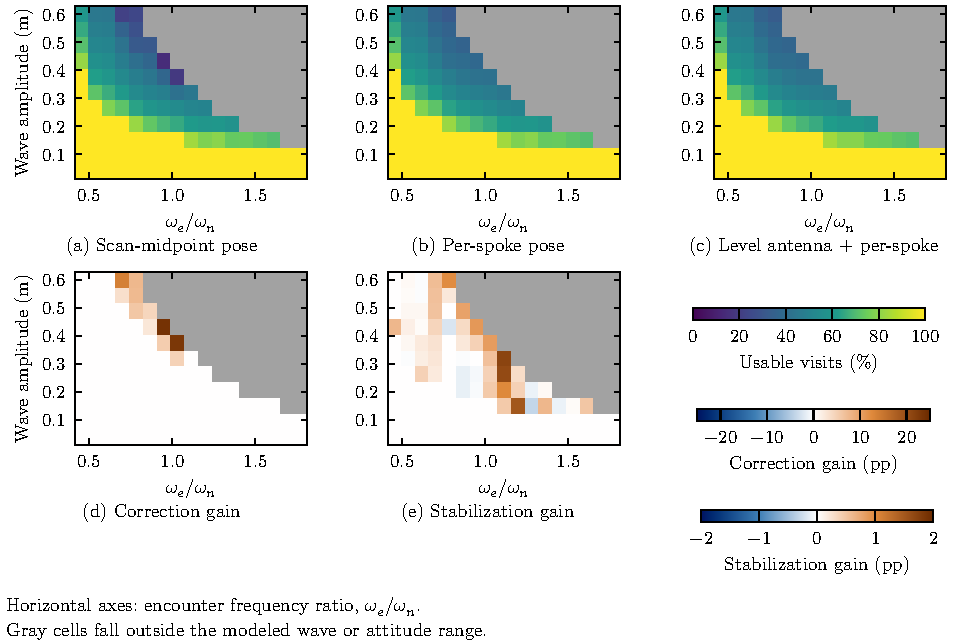
\includegraphics[width=\textwidth]{figures/operating/operating-map.pdf}
  \caption{Screened operating map of regular-wave conditions. Panels (a)--(c) report the usable fraction over 6,144 scheduled visits per cell for each method. Panels (d) and (e) give the paired gains from pose correction and level pointing in percentage points on different labeled scales. The gray cells fall outside the wave or attitude limits.}
  \label{fig:operating-map}
\end{figure*}



\subsection{Operating limits}

All three mapped arms gave 100\% usability in 50 of 111 forward, zero-yaw regular-wave cells (Fig.~\ref{fig:operating-map}). Timing correction recovered positions in 11 cells. The maximum gain was $23.76\pm0.41$ points at 0.3325 Hz and 0.432 m amplitude. Of 6,144 visits, 61.95\% had no echo, 23.76\% yielded an echo outside tolerance with the midpoint pose, and 14.29\% yielded a usable position. Correcting both pose components raised usability to 38.05\% and reduced the 95th percentile of consecutive misses from 22 visits to four.

Leveling after registration changed usability by $-0.31\pm0.12$ to $+1.71\pm0.41$ points across the grid. The tilted antenna sometimes pointed closer to the buoy. At 0.4475 Hz and 0.152 m, leveling lost 19 near-threshold echoes. In the separate reference neighborhood at fixed 0.150 m amplitude, the gain fell from 8.97 to 7.03 to zero points at 0.345, 0.350, and 0.355 Hz. Intervals describe individual cells and exclude uncertainty from selecting a maximum.

We multiplied the acquisition and position-pass fractions over all scheduled visits to test independence. The product matched midpoint usability in 100 of 111 cells, underestimated it in seven, and overestimated it in four by up to 3.75 percentage points. At 0.30375 Hz and 0.488 m, it raised the estimated registration gain from 4.39 to 13.51 percentage points. Resampling whole phase records gave a 95\% overstatement interval of 9.02--9.20 points. Both noiseless spoke-time arms factorized exactly because registration always passed.

\subsection{Interaction between pointing and registration}

Table~\ref{tab:four-arms} compares all four combinations. To isolate stand-alone interventions, we also mapped level-pointed echoes with the midpoint origin and level axes. Ranking the stand-alone gains changed the preferred first intervention in five of 111 cells relative to ranking registration against the additional gain of leveling after registration. In each, leveling led by 0.31--0.85 percentage points. At 0.36125 Hz and 0.376 m, leveling alone gained 24.01 points, recovering 1,421 positions from echoes both policies acquired and 54 from newly acquired echoes. With spoke-time registration already applied, leveling recovered those 54 echoes and lost two, yielding 0.85 points. The interaction was $-23.16$ percentage points because either intervention corrected much of the same mapping error. At 90-degree bearing in the largest registration-gain wave, leveling with the midpoint origin instead moved 692 acquired positions outside tolerance and recovered three new echoes.

\begin{table}[tb]
\caption{Usable positions out of 6,144 scheduled visits per wave. Columns cross antenna pointing with registration time.}\label{tab:four-arms}
\centering\small
\begin{tabular}{@{}lrrrr@{}}
\toprule
 & \multicolumn{2}{c}{Body-fixed} & \multicolumn{2}{c}{Level}\\
\cmidrule(lr){2-3}\cmidrule(l){4-5}
Wave (Hz, m) & Midpoint & Spoke & Midpoint & Spoke \\
\midrule
0.3500, 0.150 & 5,712 & 5,712 & 6,144 & 6,144 \\
0.3325, 0.432 & 878 & 2,338 & 2,091 & 2,392 \\
0.36125, 0.376 & 1,163 & 2,586 & 2,638 & 2,638 \\
\bottomrule
\end{tabular}
\end{table}


\subsection{Which pose component recovers an echo's position?}
At 0.3325 Hz and 0.432 m, midpoint origin and attitude gave 878 usable positions from 2,338 acquired echoes. Updating only the origin gave 1,730, only attitude gave 2,081, and both gave 2,338. The prescribed surge has the opposite sign to the free-particle horizontal orbit under our phase convention. With the original surge, none, and reversed surge, the interactions were $-18.86$, $-9.34$, and $-16.47$ points at this wave and $-23.16$, $-12.58$, and $-21.91$ points at 0.36125 Hz and 0.376 m. The reference wave gave zero interaction for every sign. The original surge mismatch reached 0.48 m against a 0.50 m tolerance. Halving surge reduced the registration gain from 23.76 to 11.59 points. Removing roll gave 4.13 points. Adding sinusoidal yaw of $1^\circ$ increased the gain to 33.35 points. Isolating bearing at an imposed 625 ms delay gave zero registration gain abeam and 32.11 points astern. With the physical crossing times below, the same bearings gave 24.28 and 24.58 points. The position test acts on the coupled motion and viewing direction.

At this forward target with 0.25 m range noise, raising the bearing standard deviation from $0.25^\circ$ to $1^\circ$ cut registration gain from 10.32 to 2.26 points.

\subsection{Common beam crossings with heading retained}

We set the rotating beam to $-90^\circ$ at each scan midpoint and solved for its crossing of the moving target bearing. The four arms shared these body-beam times. At the scan seam the pose delay wrapped to the neighboring midpoint. We tested eight bearings from $-90^\circ$ to $180^\circ$ with and without $1^\circ$ sinusoidal yaw at the wave frequency. Level pointing retained yaw at the assigned pose time.

At zero yaw the original forward counts were recovered with the quarter-scan clock. Solving the crossing changed the forward interaction from $-23.16$ to $-23.19$ points at 0.36125 Hz and 0.376 m. With yaw retained, the stand-alone leveling gain fell from 24.06 to $-1.86$ points, and the interaction became $+2.73$ points. At bearings $(-90,0,45,89.5,90,90.5,135,180)^\circ$, zero-yaw crossing interactions in this wave were $(0,-23.19,-0.47,-7.91,-2.70,-4.25,+13.33,-23.08)$ points. At $135^\circ$ leveling alone lost 13.33 points, reversing the interaction even without yaw. Adding yaw cut the forward body-midpoint usable count from 1,161 to 197 of 6,144 and raised the pose-only gain from 23.19 to 38.43 points. In the reference wave the count fell from 5,712 to 696 and timing alone gained 82.03 points, while the interaction reached $+6.64$ points. Crossing shifts were at most 10.8 ms. The stale heading can therefore govern the benefit of a level mount even when the spoke time changes little.


\subsection{Does the path model change the pointing decision?}
At the reference wave, diffraction gave 92.97\% acquisition for body pointing and 100\% for level pointing. A direct-ray visibility gate gave 100\% for both. The simulated 7.03-point benefit arose on geometrically clear rays near a crest. Adding Gaussian fluctuations to power margin reduced the expected gain to 2.41 points at 1 dB standard deviation and 1.37 at 3 dB. At the strongest registration cell diffraction gave 38.05\% for body pointing, 38.93\% for level pointing, and 38.98\% with zero angular loss. A clear-ray gate gave 42.27\% for every policy. Consequently even ideal steering recovers fewer than one extra visit per hundred there under the effective-edge model.

We also replaced the effective edge with one edge per local water crest. The Deygout construction selects the largest Fresnel--Kirchhoff parameter on each subpath, splits at that crest, and sums the resulting losses \cite{DeMinco2025Diffraction}. At the reference wave, restricting the single edge to a crest reduced the leveling gain from 7.03 to 3.13 percentage points. Including the remaining crests reduced it to 0.39 points. In the wave with the largest original registration gain, the multiple-edge model gave 10.12 points from registration and another 4.72 points from leveling. The separated-crest model changed the gain magnitudes and preserved the intervention ordering in these two waves.

As a separate sensitivity, we replaced diffraction with a direct ray and a specular ray from a horizontal plane at the buoy's instantaneous water level. Each ray used its departure angle. Reciprocal return power followed the fourth power of the summed field magnitude \cite{Galati2020Multipath}. Sweeping reflection magnitudes from zero to one and phases in $5^\circ$ steps gave leveling gains after spoke-time registration of zero to 32.42 points at the reference and zero to 32.49 at the largest-interaction wave. Both ranges collapsed to zero at $180^\circ$ reflection phase.


\subsection{Timing and precision requirements}
To compare against a system that already timestamps each spoke, we repeated all 111 grid cells with common Gaussian range and bearing errors (standard deviations 0.25 m and $0.25^\circ$). Median gains from replacing pose ages of 50, 100, 200, and 625 ms with exact timing were 0.07, 0.16, 0.49, and 3.37 percentage points, respectively. The corresponding maxima were 0.62, 1.03, 3.11, and 12.30 points. These are equally weighted grid summaries. Delay is a controlled input and requires measurement on the installed system.

At the strongest registration cell, delaying the assigned pose by up to 0.40 s at the sampled delays left all 2,338 acquired echoes within tolerance. At 0.50 s, 627 fell outside, and at 0.625 s the delay reproduced all 1,460 midpoint failures. For the $8.28^\circ$ peak pitch, Eq.~\eqref{eq:pose-delay} gives peak pitch mismatches of $6.7^\circ$ and $8.3^\circ$ at 0.40 and 0.50 s, respectively. The counting threshold depends on the phase of the echoes that survive.

At the reference wave the gain from leveling after timing correction was 1.56, 7.03, and 0.00 points at 5, 10, and 15 dB clear margin. Redistributing the reference elevation variance over seven frequencies reduced it to $0.59\pm0.19$ points and left no registration gain. The corresponding frequency ratios are $(0.72,0.83,0.92,1,1.08,1.18,1.29)$ with variance fractions $(0.08,0.13,0.19,0.23,0.19,0.12,0.06)$.
